
\documentclass{beamer}
\usecolortheme{dove}
\setbeamertemplate{navigation symbols}{}
\usepackage{amsmath,amssymb,amsfonts,amsthm, multicol, subfigure, color}
\usepackage{bm}
\usepackage{graphicx}
\usepackage{tabularx}
\usepackage{booktabs}
\usepackage{hyperref}
\usepackage{pdfpages}
\usepackage{xcolor}
\definecolor{seagreen}{RGB}{46, 139, 87}
\def\independenT#1#2{\mathrel{\rlap{$#1#2$}\mkern2mu{#1#2}}}
\newcommand\indep{\protect\mathpalette{\protect\independenT}{\perp}}
\def\log{\text{log}}
\newcommand\logit{\text{logit}}
\newcommand\iid{\stackrel{\text{iid}}{\sim}}
\newcommand\E{\text{E}}
\newcommand\V{\text{V}}
\renewcommand\P{\text{P}}
\newcommand{\Cov}{\text{Cov}}
\newcommand{\Cor}{\text{Cor}}
\newcommand\doop{\texttt{do}}
\usepackage{stackrel}
\usepackage{tikz}
\usetikzlibrary{arrows,shapes.arrows,positioning,shapes,patterns,calc}
\newcommand\slideref[1]{\vskip .1cm \tiny \textcolor{gray}{{#1}}}
\newcommand\red[1]{\color{red}#1}
\newcommand\blue[1]{\color{blue}#1}
\newcommand\gray[1]{\color{gray}#1}
\newcommand\seagreen[1]{\color{seagreen}#1}
\newcommand\purple[1]{\color{purple}#1}
\newcommand\orange[1]{\color{orange}#1}
\newcommand\black[1]{\color{black}#1}
\newcommand\white[1]{\color{white}#1}
\newcommand\teal[1]{\color{teal}#1}
\newcommand\magenta[1]{\color{magenta}#1}
\newcommand\Fuchsia[1]{\color{Fuchsia}#1}
\newcommand\BlueGreen[1]{\color{BlueGreen}#1}
\newcommand\bblue[1]{\textcolor{blue}{\textbf{#1}}}
\newcommand\bred[1]{\textcolor{red}{\textbf{#1}}}
\newcommand\bgray[1]{\textcolor{gray}{\textbf{#1}}}
\newcommand\bgreen[1]{\textcolor{seagreen}{\textbf{#1}}}
\newcommand\bref[2]{\href{#1}{\color{blue}{#2}}}
\colorlet{lightgray}{gray!40}
\pgfdeclarelayer{bg}    % declare background layer for tikz
\pgfsetlayers{bg,main} % order layers for tikz
\newcommand\mycite[1]{\begin{scriptsize}\textcolor{darkgray}{(#1)}\end{scriptsize}}
\newcommand{\tcframe}{\frame{
%\small{
\only<1|handout:0>{\tableofcontents}
\only<2|handout:1>{\tableofcontents[currentsubsection]}}
%}
}

\usepackage[round]{natbib}
\bibliographystyle{humannat-mod}
\setbeamertemplate{enumerate items}[default]
\usepackage{mathtools}

% Need to add examples

\newcommand{\goalsframe}{\begin{frame}{Learning goals for today}
At the end of class, you will be able to:
\begin{enumerate}
\item Define controlled direct effects
\item Connect them to longitudinal treatments
\item Built intuition for a new estimator: sequential $g$-estimation
\end{enumerate} \vskip .2in
\end{frame}}

\title{17. Mediation: Controlled Direct Effects.}
\author{Ian Lundberg\\Cornell Info 6751: Causal Inference in Observational Settings\\Fall 2022}
\date{20 Oct 2022}

\begin{document}

\maketitle

\goalsframe

\begin{frame}

\begin{center}
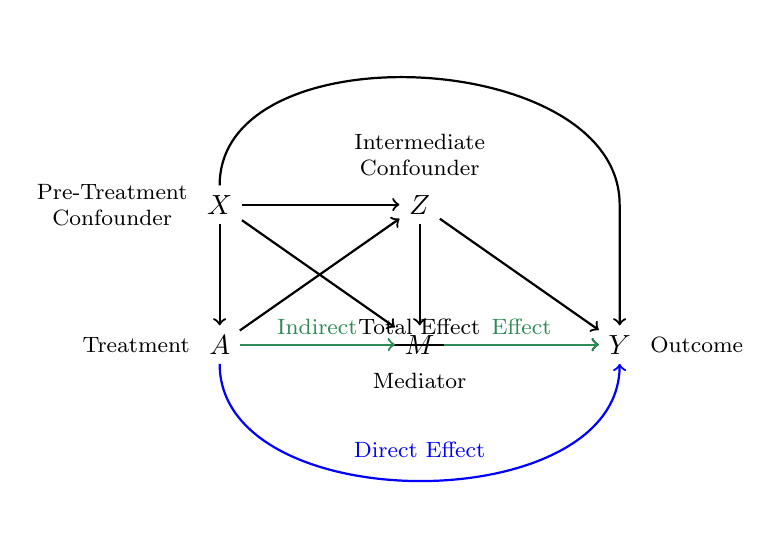
\begin{tikzpicture}[x = 1in, y = .7in]
\node (a) at (0,0) {$A$};
\node[anchor = east, font = \footnotesize] at (a.west) {Treatment};
\node (y) at (2,0) {$Y$};
\draw<1>[->, thick] (a) -- node[midway, above, font = \footnotesize] {Total Effect} (y);
\node[anchor = west, font = \footnotesize] at (y.east) {Outcome};
\onslide<2->{
\node (m) at (1,0) {$M$};
\node[anchor = north, font = \footnotesize] at (m.south) {Mediator};
\draw[->, thick, blue] (a) to[bend right = 90] node[midway, above, font = \footnotesize, outer sep = 5pt] {Direct Effect} (y);
\draw[->, thick, seagreen] (a) -- node[midway, above, font = \footnotesize, seagreen] {Indirect} (m);
\draw[->, thick, seagreen] (m) -- node[midway, above, font = \footnotesize, seagreen] {Effect} (y);
}
\onslide<3->{
\node (x) at (0,1) {$X$};
\node[anchor = east, font = \footnotesize, align = center] at (x.west) {Pre-Treatment\\Confounder};
\draw[->, thick] (x) -- (a);
\draw[->, thick] (x) -- (m);
\draw[->, thick] (x) to[out = 90, in = 90] (2,1) -- (y);
}
\onslide<4->{
\node (z) at (1,1) {$Z$};
\draw[->, thick] (a) -- (z);
\draw[->, thick] (x) -- (z);
\draw[->, thick] (z) -- (m);
\draw[->, thick] (z) -- (y);
\node[anchor = south, font = \footnotesize, align = center] at (z.north) {Intermediate\\Confounder};
}
\end{tikzpicture}
\end{center}
\onslide<5->{Before formally defining direct effects, we need a new tool}

\end{frame}

\begin{frame}{Single World Intervention Graphs (SWIGs)}{Richardson \& Robins 2013}

\begin{center}
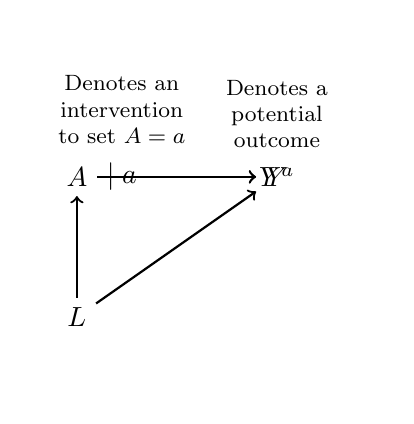
\begin{tikzpicture}[x = 1in, y = .7in]
\node at (-.2,-1.5) {};
\node at (1.5,1) {};
\onslide<2->{
\node (A) at (0,0) {$A$};
\node (L) at (0,-1) {$L$};
\draw[->, thick] (L) -- (A);
}
\node<2> (Y) at (1,0) {$Y$};
\draw<2>[->, thick] (A) -- (Y);
\draw<2->[->, thick] (L) -- (Y);
\node<3->[anchor = west] (a) at (A.east) {$\mid a$};
\node<3-> (Ya) at (1,0) {$Y^a$};
\draw<3->[->, thick] (a) -- (Y);
\node<4->[anchor = south, font = \footnotesize, align = center] at (a.north) {Denotes an\\intervention\\to set $A = a$};
\node<5->[anchor = south, font = \footnotesize, align = center] at (Ya.north) {Denotes a\\potential\\outcome};
\end{tikzpicture}
\end{center}
\onslide<6->{
SWIGs help in at least two settings:
\begin{enumerate}
\item When causal assumptions differ for each potential outcome
\item When we want to focus on a particular intervention
\end{enumerate}
}

\end{frame}

\begin{frame}{SWIGs help (1): When causal assumptions differ for each potential outcome}

\onslide<2->{
Suppose an unobserved $U$ affects the treatment $A$
} 
\vskip .1in
\onslide<3->{
\begin{tikzpicture}[x = 1in, y = .4in]
\node[anchor = north west, align = left] at (-.2,2) {Suppose $U$ affects $Y^1$};
\node (A) at (0,0) {$A$};
\node (L) at (0,-1) {$L$};
\draw[->, thick] (L) -- (A);
\draw[->, thick] (L) -- (Y);
\node[anchor = west] (1) at (A.east) {$\mid 1$};
\node (Ya) at (1,0) {$Y^1$};
\draw[->, thick] (a) -- (Y);
\node[red] (u) at (0,1) {$U$};
\draw[->, thick, red] (u) -- (Ya);
\draw[->, thick, red] (u) -- (A);
\end{tikzpicture}
}
\onslide<4->{
\begin{tikzpicture}[x = 1in, y = .4in]
\node[anchor = north west] at (-.2,2) {But $U$ does not affect $Y^0$};
\node (A) at (0,0) {$A$};
\node (L) at (0,-1) {$L$};
\draw[->, thick] (L) -- (A);
\draw[->, thick] (L) -- (Y);
\node[anchor = west] (1) at (A.east) {$\mid 0$};
\node (Ya) at (1,0) {$Y^0$};
\draw[->, thick] (a) -- (Y);
\node[red] (u) at (0,1) {$U$};
\draw[->, thick, red] (u) -- (A);
\end{tikzpicture}
} \vskip .1in
\onslide<5->{In this case, $\E(Y^1)$ is not identified but $\E(Y^0)$ is identified.}
\begin{itemize}
\onslide<6->{\item The ATC $\E(Y^1 - Y\mid A = 0)$ is not identified}
\onslide<7->{\item The ATT $\E(Y - Y^0\mid A = 1)$ is identified}
\end{itemize}
\end{frame}

\begin{frame}{SWIGs help (2): When we want to focus on a particular intervention}
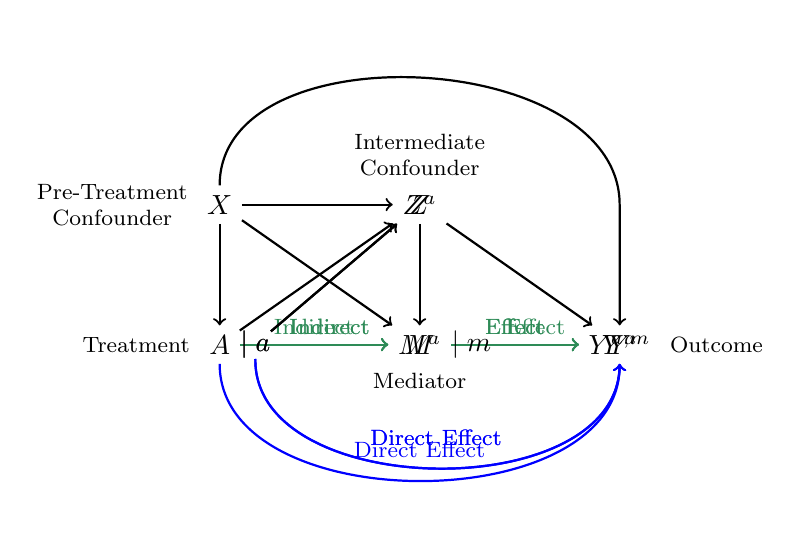
\begin{tikzpicture}[x = 1in, y = .7in]
\node (A) at (0,0) {$A$};
\node[anchor = east, font = \footnotesize] at (A.west) {Treatment};
\node<1> (y) at (2,0) {$Y$};
\node<2> (y) at (2,0) {$Y^a$};
\node<3-> (y) at (2,0) {$Y^{a,m}$};
\node[anchor = west, font = \footnotesize] at (y.east) {Outcome};
\node<1> (M) at (1,0) {$M$};
\node<2-> (M) at (1,0) {$M^a$};
\node[anchor = north, font = \footnotesize] at (M.south) {Mediator};
\node (x) at (0,1) {$X$};
\node[anchor = east, font = \footnotesize, align = center] at (x.west) {Pre-Treatment\\Confounder};
\draw[->, thick] (x) -- (A);
\draw[->, thick] (x) -- (M);
\draw[->, thick] (x) to[out = 90, in = 90] (2,1) -- (y);
\node<1> (z) at (1,1) {$Z$};
\node<2-> (z) at (1,1) {$Z^a$};
\draw[->, thick] (x) -- (z);
\draw[->, thick] (z) -- (M);
\draw[->, thick] (z) -- (y);
\node[anchor = south, font = \footnotesize, align = center] at (z.north) {Intermediate\\Confounder};
\draw<1-2>[->, thick, seagreen] (M) -- node[midway, above, font = \footnotesize, seagreen] {Effect} (y);
\onslide<1>{
\draw[->, thick, blue] (A) to[bend right = 90] node[midway, above, font = \footnotesize, outer sep = 5pt] {Direct Effect} (y);
\draw[->, thick, seagreen] (A) -- node[midway, above, font = \footnotesize, seagreen] {Indirect} (M);
\draw[->, thick] (A) -- (z);
}
\onslide<2>{
\node[anchor = west, inner sep = 0pt] (a) at (A.east) {$\mid a$};
\draw[->, thick, seagreen] (M) -- node[midway, above, font = \footnotesize, seagreen] {Effect} (y);
\draw[->, thick, blue] (a) to[bend right = 90] node[midway, above, font = \footnotesize, outer sep = 5pt] {Direct Effect} (y);
\draw[->, thick, seagreen] (a) -- node[midway, above, font = \footnotesize, seagreen] {Indirect} (M);
\draw[->, thick] (a) -- (z);
}
\onslide<3->{
\node[anchor = west, inner sep = 0pt] (a) at (A.east) {$\mid a$};
\node[anchor = west, inner sep = 0pt] (m) at (M.east) {$\mid m$};
\draw[->, thick, seagreen] (m) -- node[midway, above, font = \footnotesize, seagreen] {Effect} (y);
\draw[->, thick, blue] (a) to[bend right = 90] node[midway, above, font = \footnotesize, outer sep = 5pt] {Direct Effect} (y);
\draw[->, thick, seagreen] (a) -- node[midway, above, font = \footnotesize, seagreen] {Indirect} (M);
\draw[->, thick] (a) -- (z);
}
\end{tikzpicture}
\end{frame}

\begin{frame}{Controlled direct effect (CDE)}
\begin{tikzpicture}[x = \textwidth, y = .8\textheight]
\node at (0,0) {};
\node at (1,1) {};
\node[anchor = north east] at (1,1) {\scalebox{.5}{\begin{tikzpicture}[x = 1in, y = .7in, every node/.style = {anchor=center}]
\node (A) at (0,0) {$A$};
\node[anchor = east, font = \footnotesize] at (A.west) {Treatment};
\node (y) at (2,0) {$Y^{a,m}$};
\node[anchor = west, font = \footnotesize] at (y.east) {Outcome};
\node (M) at (1,0) {$M^a$};
\node[anchor = north, font = \footnotesize] at (M.south) {Mediator};
\node (z) at (1,1) {$Z^a$};
\node (x) at (0,1) {$X$};
\node[anchor = east, font = \footnotesize, align = center] at (x.west) {Pre-Treatment\\Confounder};
\draw[->, thick] (x) -- (A);
\draw[->, thick] (x) -- (M);
\draw[->, thick] (x) to[out = 90, in = 90] (2,1) -- (y);
\draw[->, thick] (x) -- (z);
\draw[->, thick] (z) -- (M);
\draw[->, thick] (z) -- (y);
\node[anchor = south, font = \footnotesize, align = center] at (z.north) {Intermediate\\Confounder};
\node[anchor = west, inner sep = 0pt] (a) at (A.east) {$\mid a$};
\node[anchor = west, inner sep = 0pt] (m) at (M.east) {$\mid m$};
\draw[->, thick, seagreen] (m) -- node[midway, above, font = \footnotesize, seagreen] {Effect} (y);
\draw[->, thick, blue] (a) to[bend right = 90] node[midway, above, font = \footnotesize, outer sep = 5pt] {Direct Effect} (y);
\draw[->, thick, seagreen] (a) -- node[midway, above, font = \footnotesize, seagreen] {Indirect} (M);
\draw[->, thick] (a) -- (z);
\end{tikzpicture}}};
% Begin equations
\node<2->[anchor = west] at (0,.6) {Definition: Controlled Direct Effect};
\node<2->[anchor = west] at (0,.5) {$\tau(m) = \E\left(Y^{1,m} - Y^{0,m}\right)$};
\node<2->[anchor = north west, align = left] at (0,.4) {The effect of an intervention to set treatment $A = 1$ vs $A = 0$\\
while also intervening to set the mediator to $M = m$};
\end{tikzpicture}
\end{frame}

\begin{frame}{CDE in an experiment}

You are an elementary school principal \vskip .2in

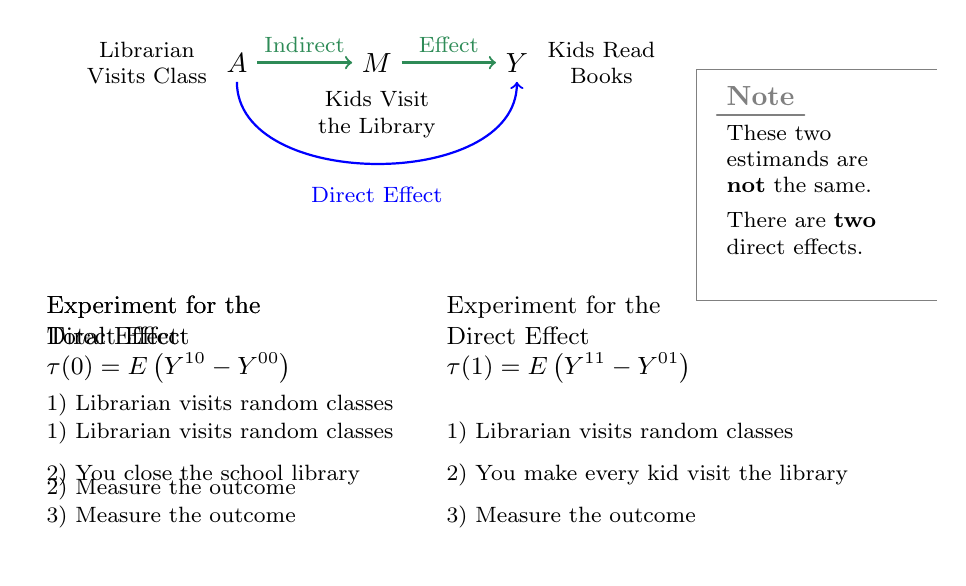
\begin{tikzpicture}[x = 1in, y = .7in, every node/.style = {anchor=center}]
\node at (-1,-1.6) {};
\onslide<2->{
\node (y) at (1.4,0) {$Y$};
\node[anchor = west, font = \footnotesize, align = center] at (y.east) {Kids Read\\Books};
}
\onslide<3->{
\node (A) at (0,0) {$A$};
\node[anchor = east, font = \footnotesize, align = center] at (A.west) {Librarian\\Visits Class};
}
\onslide<4->{
\node (M) at (.7,0) {$M$};
\node[anchor = north, font = \footnotesize, align = center] at (M.south) {Kids Visit\\the Library};
\draw[->, thick, seagreen] (A) -- node[midway, above, font = \footnotesize, seagreen] {Indirect} (M);
\draw[->, thick, seagreen] (M) -- node[midway, above, font = \footnotesize, seagreen] {Effect} (y);
}
\onslide<5->{
\draw[->, thick, blue] (A) to[bend right = 90] node[midway, below, font = \footnotesize, outer sep = 5pt] {Direct Effect} (y);
}
\node<6-8>[anchor = north west, font = \small, align = left] at (-1,-1.6) {Experiment for the\\Total Effect};
\node<7-8>[anchor = north west, font = \footnotesize] at (-1,-2.3) {1) Librarian visits random classes};
\node<8>[anchor = north west, font = \footnotesize] at (-1,-2.9) {2) Measure the outcome};
\node<9->[anchor = north west, font = \small, align = left] at (-1,-1.6) {Experiment for the\\Direct Effect\\$\tau(0) = E\left(Y^{10} - Y^{00}\right)$};
\node<10->[anchor = north west, font = \footnotesize] at (-1,-2.5) {1) Librarian visits random classes};
\node<11->[anchor = north west, font = \footnotesize] at (-1,-2.8) {2) You close the school library};
\node<13->[anchor = north west, font = \footnotesize] at (-1,-3.1) {3) Measure the outcome};
\node<9->[anchor = north west, font = \small, align = left] at (1,-1.6) {Experiment for the\\Direct Effect\\$\tau(1) = E\left(Y^{11} - Y^{01}\right)$};
\node<10->[anchor = north west, font = \footnotesize] at (1,-2.5) {1) Librarian visits random classes};
\node<12->[anchor = north west, font = \footnotesize] at (1,-2.8) {2) You make every kid visit the library};
\node<13->[anchor = north west, font = \footnotesize] at (1,-3.1) {3) Measure the outcome};
\node[anchor = north west, font = \footnotesize] at (1,-3.4) {};
\node<14->[anchor = north west, align = left, font = \footnotesize, color = gray, font = \bf] (imp) at (2.4,-.1) {\textbf{Note}};
\draw<14->[thick, gray, line cap = round] (imp.south west) -- (imp.south east);
\node<14->[anchor = north west, align = left, font = \footnotesize] (impnote) at (imp.south west) {These two\\estimands are\\\textbf{not} the same.};
\node<14->[anchor = north west, align = left, font = \footnotesize] (impnote2) at (impnote.south west) {There are \textbf{two}\\direct effects.};
\draw<14->[gray] (3.5,-.05) -- (2.3,-.05) -- (2.3,-1.7) -- (3.5,-1.7); 
\end{tikzpicture}

\end{frame}

\begin{frame}{CDE warning: Non-manipulable mediators} \pause

It is hard to study mediators that occur inside a person's head\vskip .1in
  \pause
\begin{itemize}
\item Psychological stimulus $\rightarrow$ Stress $\rightarrow$ Test performance \pause
\item Exposure to racial outgroup $\rightarrow$ Racial resentment $\rightarrow$ Voting \pause
\item Father incarcerated $\rightarrow$ Mother depressed $\rightarrow$ Child behavior \pause
\end{itemize} \vskip .1in
No experiment could manipulate these mediators \vskip .2in \pause
Mediators outside a person's head are easier to study
\begin{itemize}
\item Example: Require every kid to visit the school library
\end{itemize}

\end{frame}

\begin{frame}

CDE identification and estimation in observational studies

\end{frame}

\begin{frame}{A visual summary: Nonparametric sequential $g$-estimation}{Estimating $\tau(0) = \E(Y^{10} - Y^{00})$}
\begin{tikzpicture}[x = \textwidth, y = .6\textheight, every node/.style = {font = \footnotesize}]
\node at (0,0) {};
\node at (1,1.1) {};
\node [anchor = north west, align = left] at (0,1.3) {Text here will tell the story for those reading these slides online.};
\end{tikzpicture}
\end{frame}

\begin{frame}{A visual summary: Nonparametric sequential $g$-estimation}{Estimating $\tau(0) = \E(Y^{10} - Y^{00})$}
\begin{tikzpicture}[x = \textwidth, y = .6\textheight, every node/.style = {font = \footnotesize}]
\node at (0,0) {};
\node at (1,1.1) {};
\node<1> [anchor = north west, align = left] at (0,1.3) {Treatment variable $A$.\\You can think of this as randomized, or you can take this entire story to\\take place within subgroups of $\vec{X}$ sufficient to yield exchangeability.};
\node<2> [anchor = north west] at (0,1.3) {$A$ affects an intermediate confounder $Z$};
\node<3> [anchor = north west] at (0,1.3) {$Z$ affects the mediator $M$};
\node<4-9> [anchor = north west, align = left] at (0,1.3) {We observe outcome means $\bar{Y}$ in each subgroup.\\We can now impute the outcome $Y^{A0}$ under $M = 0$\\in each stratum of $\{A,Z\}$.};
\node<10> [anchor = north west, align = left] at (0,1.3) {To focus on the effect of $A$, we now ignore $Z$.};
\node<11-13> [anchor = north west, align = left] at (0,1.3) {To focus on the effect of $A$, we now ignore $Z$.\\We have a weighted average over $Z\mid A = a$ for each $a$.\\Because the effect of $A$ is identified, $\underbrace{(Z\mid A = a)}_\text{Observational}\quad\sim \underbrace{(Z^a)}_\text{Interventional}$};
\node<14> [anchor = north west, align = left] at (0,1.3) {The difference is the CDE $\tau(0)$!};
\onslide<1->{
\node at (.2,.75) {$A = 0$};
\node at (.2,.25) {$A = 1$};
\draw (.1, .5) rectangle (.3, 1);
\draw (.1, .5) rectangle (.3, 0);
% Example
\node[anchor = north west, gray, font = \tiny, align = left] at (.1,1) {Librarian\\does not\\visit class};
\node[anchor = north west, gray, font = \tiny, align = left] at (.1,.5) {Librarian\\visits class};
}
\onslide<2-9>{
\node at (.4,.85) {$Z = 0$};
\node at (.4,.6) {$Z = 1$};
\node at (.4,.4) {$Z = 0$};
\node at (.4,.15) {$Z = 1$};
\draw (.3, .7) rectangle (.5, 1);
\draw (.3, .5) rectangle (.5, .7);
\draw (.3, .5) rectangle (.5, .3);
\draw (.3, .3) rectangle (.5, 0);
% Example
\node[anchor = north west, gray, font = \tiny, align = left] at (.3,1) {I'd rather play};
\node[anchor = north west, gray, font = \tiny, align = left] at (.3,.7) {I want a book!};
}
\onslide<3-5>{
\node at (.6,.9) {$M = 0$};
\draw (.5, .85) rectangle (.7, 1);
\node at (.6,.75) {$M = 1$};
\draw (.5, .7) rectangle (.7, .85);
% Example
\node[anchor = north west, gray, font = \tiny, align = left] at (.5,1) {Visits playground};
\node[anchor = north west, gray, font = \tiny, align = left] at (.5,.85) {Visits library};
}
\onslide<4-5>{
\node[anchor = north west, gray, font = \tiny, align = left] at (.7,1) {Reads books};
\draw (.7, .7) rectangle (.9, .85);
\draw (.7, .85) rectangle (.9, 1);
\draw<5>[blue, line width = 2pt] (.7, .85) rectangle (.9, 1);
\node at (.8,.9) {$\bar{Y}$};
\node at (.8,.775) {$\bar{Y}$};
}
\onslide<3-6>{
\node at (.6,.675) {$M = 0$};
\draw (.5, .65) rectangle (.7, .7);
\node at (.6,.575) {$M = 1$};
\draw (.5, .5) rectangle (.7, .65);
}
\onslide<4-6>{
\draw (.7, .65) rectangle (.9, .7);
\draw (.7, .5) rectangle (.9, .65);
\node at (.8,.675) {$\bar{Y}$};
\node at (.8,.575) {$\bar{Y}$};
}
\onslide<3-7>{
\node at (.6,.425) {$M = 0$};
\draw (.5, .5) rectangle (.7, .35);
\node at (.6,.325) {$M = 1$};
\draw (.5, .3) rectangle (.7, .35);
}
\onslide<4-7>{
\draw (.7, .5) rectangle (.9, .35);
\draw (.7, .3) rectangle (.9, .35);
\node at (.8,.425) {$\bar{Y}$};
\node at (.8,.325) {$\bar{Y}$};
}
\onslide<3-8>{
\node at (.6,.2) {$M = 0$};
\draw (.5, .1) rectangle (.7, .3);
\node at (.6,.05) {$M = 1$};
\draw (.5, 0) rectangle (.7, .1);
}
\onslide<4-8>{
\draw (.7, .1) rectangle (.9, .3);
\draw (.7, 0) rectangle (.9, .1);
\node at (.8,.2) {$\bar{Y}$};
\node at (.8,.05) {$\bar{Y}$};
}
\onslide<6-12>{
\node[anchor = north west, gray, font = \tiny, align = left] at (.5,1) {Proportion reading books if we prevent\\anyone from visiting the library ($M = 0$)};
\node at (.7,.85) {$\E(Y^{00}\mid A = 0, Z = 0)$};
\draw (.5, .7) rectangle (.9, 1);
\draw<6>[blue, line width = 2pt] (.5, .7) rectangle (.9, 1);
}
\onslide<7-12>{
\node at (.7,.6) {$\E(Y^{00}\mid A = 0, Z = 1)$};
\draw (.5, .5) rectangle (.9, .7);
}
\onslide<8-12>{
\node at (.7,.4) {$\E(Y^{10}\mid A = 1, Z = 0)$};
\draw (.5, .5) rectangle (.9, .3);
}
\onslide<9-12>{
\node at (.7,.15) {$\E(Y^{10}\mid A = 1, Z = 1)$};
\draw (.5, .3) rectangle (.9, 0);
}
\onslide<11-12>{
\node[align = center, font = \footnotesize] at (.4,.75) {Weighted by\\distribution of\\$Z\mid A = 0$};
\draw[->, thick] (.425, .85) -- (.475, .9);
\draw[->, thick] (.425, .65) -- (.475, .6);
}
\onslide<12>{
\node[align = center, font = \footnotesize] at (.4,.25) {Weighted by\\distribution of\\$Z\mid A = 1$};
\draw[->, thick] (.425, .35) -- (.475, .4);
\draw[->, thick] (.425, .15) -- (.475, .1);
}
\onslide<13->{
\node at (.6,.75) {$\E(Y^{10})$};
}
\onslide<13->{
\node at (.6,.25) {$\E(Y^{00})$};
}
\end{tikzpicture}
\end{frame}

\begin{frame}
Sometimes we want to estimate with a model
\end{frame}

\begin{frame}[t]{Parametric sequential $g$-estimation {\scriptsize (see \bref{https://doi.org/10.1017/S0003055416000216}{Acharya, Blackwell, \& Sen 2016})}} \vskip .2in
\begin{center}
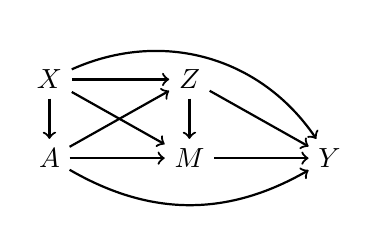
\begin{tikzpicture}[x = .7in]
\node (a) at (0,0) {$A$};
\node (m) at (1,0) {$M$};
\node (y) at (2,0) {$Y$};
\node (x) at (0,1) {$X$};
\node (z) at (1,1) {$Z$};
\draw[->, thick] (a) -- (z);
\draw[->, thick] (a) -- (m);
\draw[->, thick] (a) to[bend right] (y);
\draw[->, thick] (m) -- (y);
\draw[->, thick] (x) -- (a);
\draw[->, thick] (x) -- (m);
\draw[->, thick] (x) -- (z);
\draw[->, thick] (x) to[bend left = 40] (y);
\draw[->, thick] (z) -- (m);
\draw[->, thick] (z) -- (y);
\end{tikzpicture}
\end{center}
High-level overview: \pause
\begin{enumerate}
\item Estimate the effect of the mediator \pause
\begin{itemize}
\item Model $Y$ given $X, A, Z, M$ \pause
\end{itemize}
\item Construct $\tilde{Y}$ with the effect of the mediator removed \pause
\begin{itemize}
\item $\tilde{Y} = Y - \left[\E(Y^M\mid X, A, Z) - \E(Y^0\mid X, A, Z)\right]$ \pause
\end{itemize}
\item Estimate treatment effect on the de-mediated outcome \pause
\begin{itemize}
\item Model $\tilde{Y}$ given $X, A$
\end{itemize}
\end{enumerate}
\end{frame}

\begin{frame}[t]{Parametric sequential $g$-estimation {\scriptsize (see \bref{https://doi.org/10.1017/S0003055416000216}{Acharya, Blackwell, \& Sen 2016})}} \vskip .2in
\begin{center}
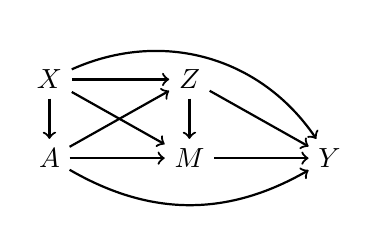
\begin{tikzpicture}[x = .7in]
\node (a) at (0,0) {$A$};
\node (m) at (1,0) {$M$};
\node (y) at (2,0) {$Y$};
\node (x) at (0,1) {$X$};
\node (z) at (1,1) {$Z$};
\draw[->, thick] (a) -- (z);
\draw[->, thick] (a) -- (m);
\draw[->, thick] (a) to[bend right] (y);
\draw[->, thick] (m) -- (y);
\draw[->, thick] (x) -- (a);
\draw[->, thick] (x) -- (m);
\draw[->, thick] (x) -- (z);
\draw[->, thick] (x) to[bend left = 40] (y);
\draw[->, thick] (z) -- (m);
\draw[->, thick] (z) -- (y);
\end{tikzpicture}
\end{center}

\bgray{Step 1:} What outcome would have been realized at each $M = m$? \vskip .1in \pause
$$\E(Y^m\mid X, A, Z) = \E(Y\mid X, A, Z, M = m)$$
because $M\rightarrow Y$ is identifiied given $\{X,A,Z\}$

\end{frame}

\begin{frame}[t]{Parametric sequential $g$-estimation {\scriptsize (see \bref{https://doi.org/10.1017/S0003055416000216}{Acharya, Blackwell, \& Sen 2016})}} \vskip .2in
\begin{center}
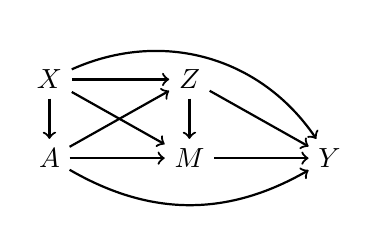
\begin{tikzpicture}[x = .7in]
\node (a) at (0,0) {$A$};
\node (m) at (1,0) {$M$};
\node (y) at (2,0) {$Y$};
\node (x) at (0,1) {$X$};
\node (z) at (1,1) {$Z$};
\draw[->, thick] (a) -- (z);
\draw[->, thick] (a) -- (m);
\draw[->, thick] (a) to[bend right] (y);
\draw[->, thick] (m) -- (y);
\draw[->, thick] (x) -- (a);
\draw[->, thick] (x) -- (m);
\draw[->, thick] (x) -- (z);
\draw[->, thick] (x) to[bend left = 40] (y);
\draw[->, thick] (z) -- (m);
\draw[->, thick] (z) -- (y);
\end{tikzpicture}
\end{center}

\bgray{Step 2:}
Construct a \bgray{de-mediated outcome} \pause
$$\tilde{Y} = Y - \gamma(X,A,M)$$
where the de-mediation function $\gamma$ is
$$\underbrace{\gamma(X,A,M)}_{\substack{\text{Not a function of $Z$}\\\text{See below}}} = \underbrace{\E(Y\mid X, A, Z, M) - \E(Y\mid X, A, Z, M = 0)}_\text{Causal effect of the factual mediator value $M$ vs 0}$$ \vskip .1in \pause

\bgray{New assumption:} No $Z\times M$ interactions {\footnotesize (simplifies estimation)}
\begin{itemize}
\item The effect $M\rightarrow Y$ does not depend on $Z$
\item By this assumption, $\gamma$ is not a function of $Z$
\end{itemize}
\end{frame}

\begin{frame}[t]{Parametric sequential $g$-estimation {\scriptsize (see \bref{https://doi.org/10.1017/S0003055416000216}{Acharya, Blackwell, \& Sen 2016})}} \vskip .2in
\begin{center}
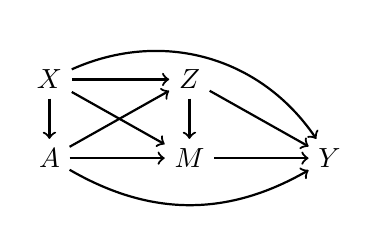
\begin{tikzpicture}[x = .7in]
\node (a) at (0,0) {$A$};
\node (m) at (1,0) {$M$};
\node (y) at (2,0) {$Y$};
\node (x) at (0,1) {$X$};
\node (z) at (1,1) {$Z$};
\draw[->, thick] (a) -- (z);
\draw[->, thick] (a) -- (m);
\draw[->, thick] (a) to[bend right] (y);
\draw[->, thick] (m) -- (y);
\draw[->, thick] (x) -- (a);
\draw[->, thick] (x) -- (m);
\draw[->, thick] (x) -- (z);
\draw[->, thick] (x) to[bend left = 40] (y);
\draw[->, thick] (z) -- (m);
\draw[->, thick] (z) -- (y);
\end{tikzpicture}
\end{center}

\bgray{Step 3:}
Estimate the treatment effect on the de-mediated outcome
$$\E(Y^{a,0}\mid X) = \E(\tilde{Y}\mid X, A = a)$$
\end{frame}

\begin{frame}[t]{Parametric sequential $g$-estimation {\scriptsize (see \bref{https://doi.org/10.1017/S0003055416000216}{Acharya, Blackwell, \& Sen 2016})}} \vskip .2in
\begin{center}
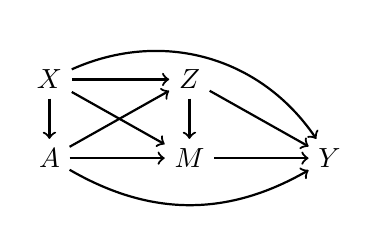
\begin{tikzpicture}[x = .7in]
\node (a) at (0,0) {$A$};
\node (m) at (1,0) {$M$};
\node (y) at (2,0) {$Y$};
\node (x) at (0,1) {$X$};
\node (z) at (1,1) {$Z$};
\draw[->, thick] (a) -- (z);
\draw[->, thick] (a) -- (m);
\draw[->, thick] (a) to[bend right] (y);
\draw[->, thick] (m) -- (y);
\draw[->, thick] (x) -- (a);
\draw[->, thick] (x) -- (m);
\draw[->, thick] (x) -- (z);
\draw[->, thick] (x) to[bend left = 40] (y);
\draw[->, thick] (z) -- (m);
\draw[->, thick] (z) -- (y);
\end{tikzpicture}
\end{center}
High-level overview:
\begin{enumerate}
\item Estimate the effect of the mediator
\begin{itemize}
\item Model $Y$ given $X, A, Z, M$
\end{itemize}
\item Construct $\tilde{Y}$ with the effect of the mediator removed
\begin{itemize}
\item $\tilde{Y} = Y - \left[\E(Y^M\mid X, A, Z) - \E(Y^0\mid X, A, Z)\right]$
\end{itemize}
\item Estimate treatment effect on the de-mediated outcome
\begin{itemize}
\item Model $\tilde{Y}$ given $X, A$
\end{itemize}
\end{enumerate}
\end{frame}

\goalsframe

\begin{frame}{Let me know what you are thinking}

\begin{huge} \bref{https://tinyurl.com/CausalQuestions}{tinyurl.com/CausalQuestions} \end{huge}
\vskip .7in

Office hours TTh 11am-12pm and at \bref{https://calendly.com/ianlundberg/office-hours}{calendly.com/ianlundberg/office-hours}\\Come say hi!

\end{frame}

\end{document}